\chapter{原型系统与案例验证}

\section{原型系统构建}
% 原型系统架构用不用写?
\subsection{网络结构}
本系统部署在4台服务器,如表~\ref{tab:server-cfg}所示,其中“172.21.213.177”服务器是南师大地科院的刀片服务器上的虚拟机,CPU是E5-2630,10个核心,支持10个IBIS模型实例并行运行;“192.168.190.128”服务器是位于本地PC机的虚拟机上,CPU是i7-4770,4个核心,支持Biome-BGC和LPJ共4个实例并行运行;“172.21.212.58”服务器也是南师大地科院的刀片服务器上的虚拟机,硬盘大小200GB,支持大容量数据快速存取;“223.2.35.73”服务器位于本地PC机,CPU是i7-4770,8个核心。这些服务器都位于同一个局域网下,保证了数据传输速度。

\begin{table}[H]
    \centering
    \caption{服务器部署配置}
    \label{tab:server-cfg}
    \begin{threeparttable}
        \begin{tabular}{lllllll}
            \Xhline{1.5pt}
            层级 & 地址 & 端口 & 部署的微服务 \\
            \Xhline{1pt}
            \multirow{3}{*}{模型计算层} & 172.21.213.177 & 6868 & IBIS服务 \\
            % \cline{2-4}
            & \multirow{2}{*}{192.168.190.128} & \multirow{2}{*}{6868} & Biome-BGC服务 \\
            % \cline{4-4}
            &&& LPJ服务 \\
            \hline
            \multirow{4}{*}{数据管理层} & \multirow{4}{*}{172.21.212.58} & \multirow{3}{*}{8786} & 数据上传服务 \\
            % \cline{4-4}
            &&& 数据下载服务 \\
            % \cline{4-4}
            &&& 数据重构服务 \\
            % \cline{3-4}
            && 8787 & WMS WFS WCS \\
            \hline
            模型对比层 & 223.2.35.73 & 9999 & 对比服务 \\
            \Xhline{1.5pt}
        \end{tabular}
    \end{threeparttable}
\end{table}

\subsection{微服务容器}
服务容器作为服务的承载工具,它本身并不处理非常复杂的计算逻辑,而是将CPU密集型操作交给它所容纳的服务,所以服务容器是IO密集型的程序,他需要处理高并发的HTTP请求。Node.js作为异步编程的代表,天生适合这种场景,所以本文选择Node.js作为后台服务容器开发语言,使用MongoDB管理数据。由于Node.js的单线程特性,它本身并不稳定,所以使用PM2进行单台服务节点上Node.js应用的负载均衡。

\begin{figure}[!htbp]
    \centering
    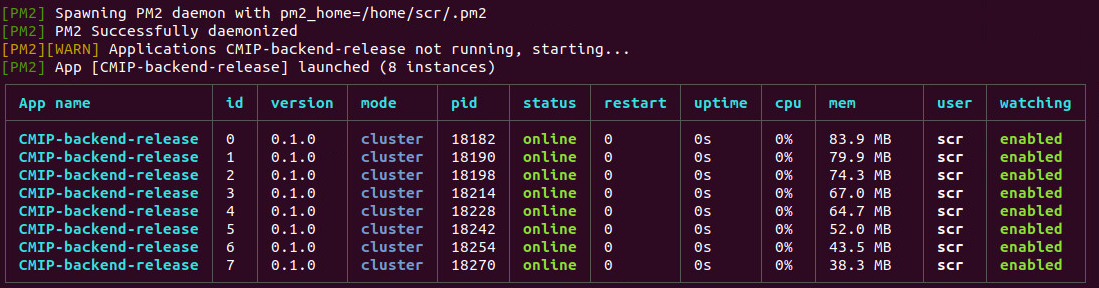
\includegraphics[width=1\textwidth]{PM2}
    \caption{PM2负载均衡管理}
    \label{fig:ms-step}
\end{figure}

微服务容器作为面向管理员的后台管理工具,数据管理容器、模型计算容器和模型对比容器都具有很多通用的功能,如图~\ref{fig:service-container-common-fn}所示,微服务容器可以对服务进行管理,包括发布、注销、实例管理等,此外,还可以对服务器性能进行监控。

\begin{figure}[!htbp]
    \centering
    \subcaptionbox{服务列表、重新发布、注销\label{fig:service-publish-removal}}{
\includegraphics[width=.48\textwidth]{ms-step}}
    \hfill
    \subcaptionbox{服务上传部署发布\label{fig:service-deploy}}{
\includegraphics[width=.48\textwidth]{ms-step}} \\
    \subcaptionbox{服务实例管理\label{fig:insitance-manage}}{
\includegraphics[width=.48\textwidth]{ms-step}}
    \hfill
    \subcaptionbox{服务器性能监测\label{fig:monitor}}{
\includegraphics[width=.48\textwidth]{ms-step}}
    \caption{微服务容器通用功能}
    \label{fig:service-container-common-fn}
\end{figure}

除了通用功能,数据管理容器通过Nginx的消息中转还支持使用GeoServer发布WMS、WFS、WCS服务(图~\ref{fig:geoserver}),模型对比容器支持对计算节点进行管理(图~\ref{fig:api-gateway-children})。

\begin{figure}[!htbp]
    \centering
    
\includegraphics[width=1\textwidth]{ms-step}
    \caption{GeoServer发布数据服务}
    \label{fig:geoserver}
\end{figure}

\begin{figure}[!htbp]
    \centering
    
\includegraphics[width=1\textwidth]{ms-step}
    \caption{API网关(对比服务容器)上注册的子节点}
    \label{fig:api-gateway-children}
\end{figure}

\subsection{陆地生态系统碳循环模型对比门户网站}
面向开放式模型计算和对比的需求,本文构建了一个门户网站,作为对比方案和对比结果共享的入口。一方面可以将对比过程和结果公开化,降低碳循环模型的使用难度,另一方面可以激励模式组的模型通过封装加入进来,促进碳循环研究的发展。门户网站的主要功能模块设计为如图\ref{fig:system-module},功能模块分为资源模块、对比业务模块、结果展示模块和用户管理模块,其中资源模块包括模型资源和数据资源;对比业务模块则对应于对比话题、对比方案和对比任务;结果展示模块基于所有对比任务的执行结果,将对比结果展示出去;用户模块包括用户的个人资源管理。门户网站的登录、注册和首页如图~\ref{fig:portal-index}所示。

\begin{figure}[!htbp]
    \centering
    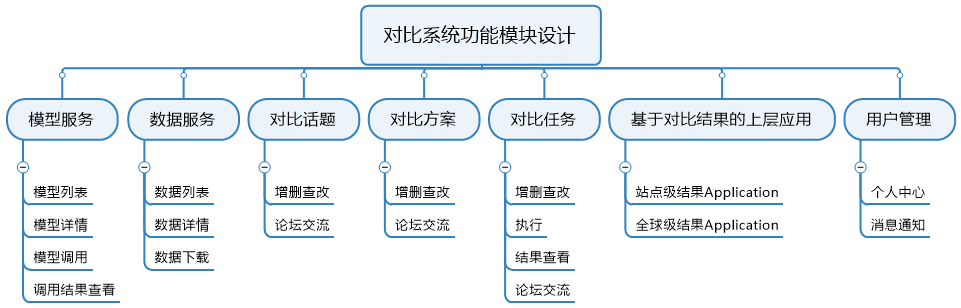
\includegraphics[width=1\textwidth]{system-module}
    \caption{对比系统功能模块设计}
    \label{fig:system-module}
\end{figure}

\begin{figure}[!htbp]
    \centering
    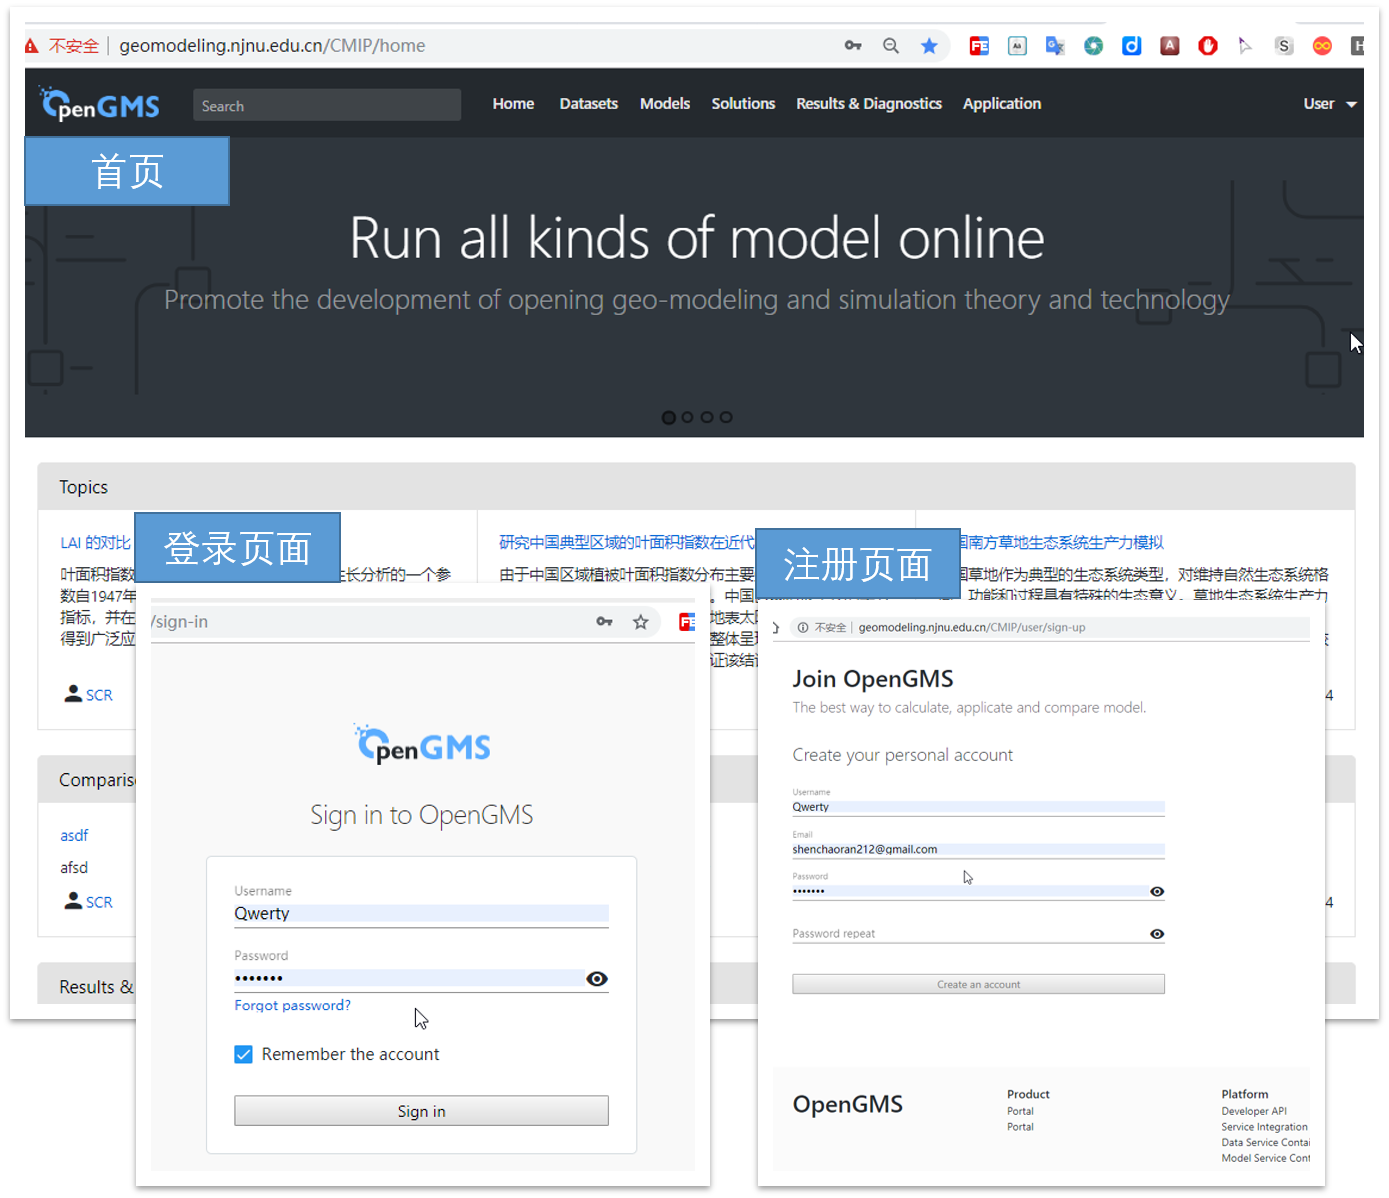
\includegraphics[width=.7\textwidth]{portal-index}
    \caption{门户网站首页和注册登录页面}
    \label{fig:portal-index}
\end{figure}

\begin{figure}[!htbp]
    \centering
    \subcaptionbox{模型资源和数据资源列表\label{fig:ms-data-resource}}{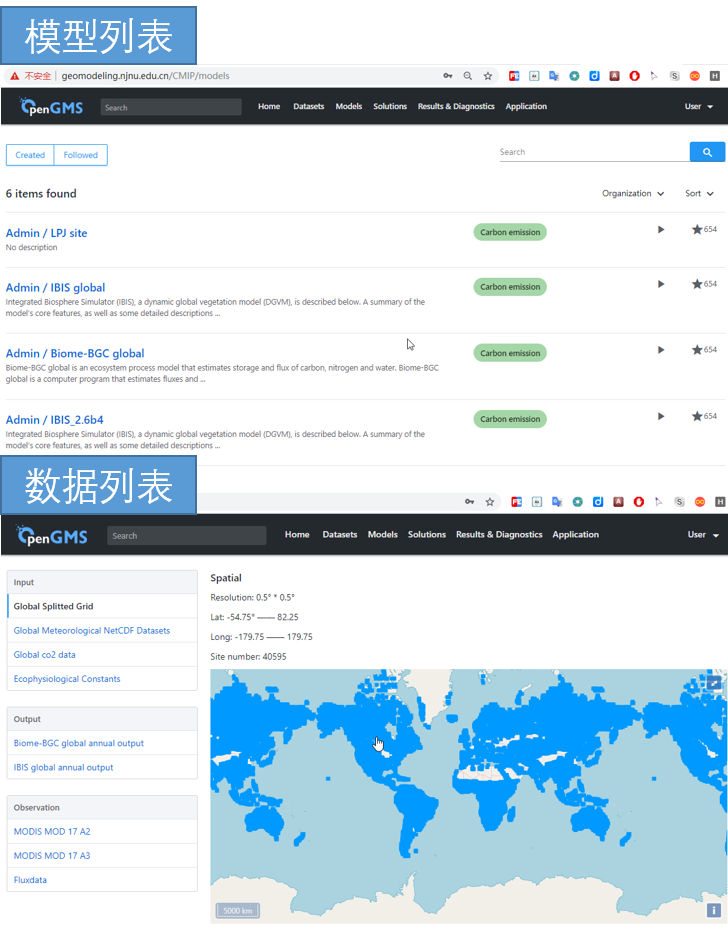
\includegraphics[width=.5\textwidth]{ms-data-resource}}
    \hfill
    \subcaptionbox{模型服务调用\label{fig:ms-invoke}}{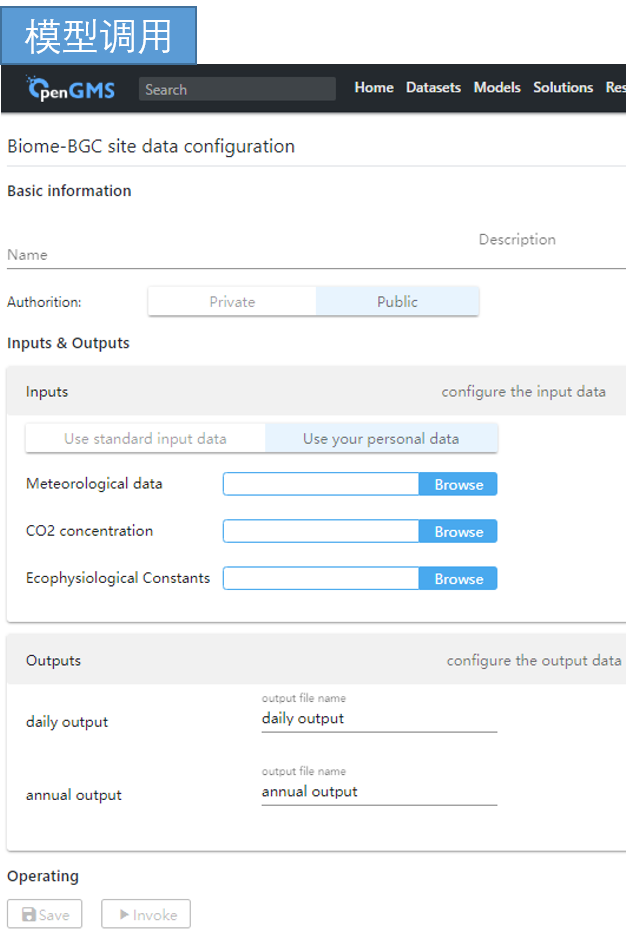
\includegraphics[width=.43\textwidth]{ms-invoke}}
    \caption{门户网站模型和数据资源}
    \label{fig:portal-resource}
\end{figure}

\begin{figure}[!htbp]
    \centering
    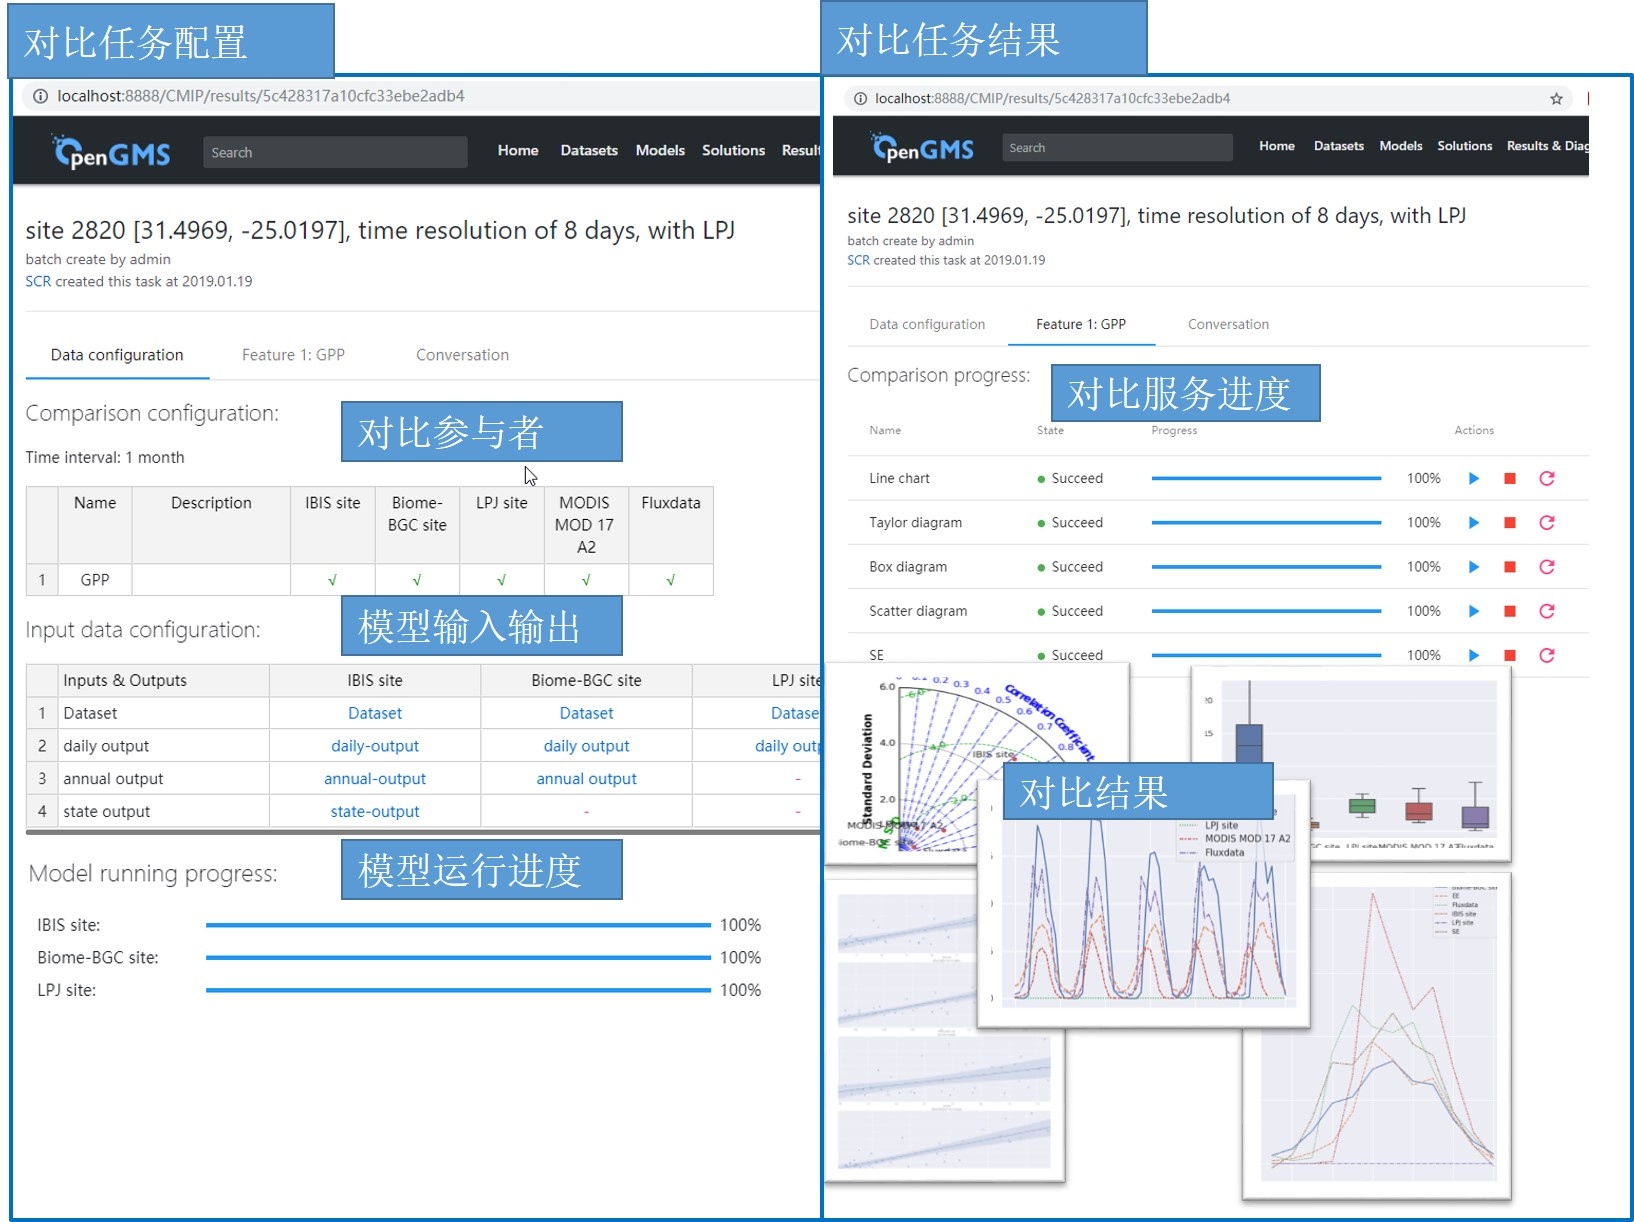
\includegraphics[width=1\textwidth]{task-cfg-result}
    \caption{对比任务配项和结果}
    \label{fig:task-cfg-result}
\end{figure}

\begin{figure}[!htbp]
    \centering
    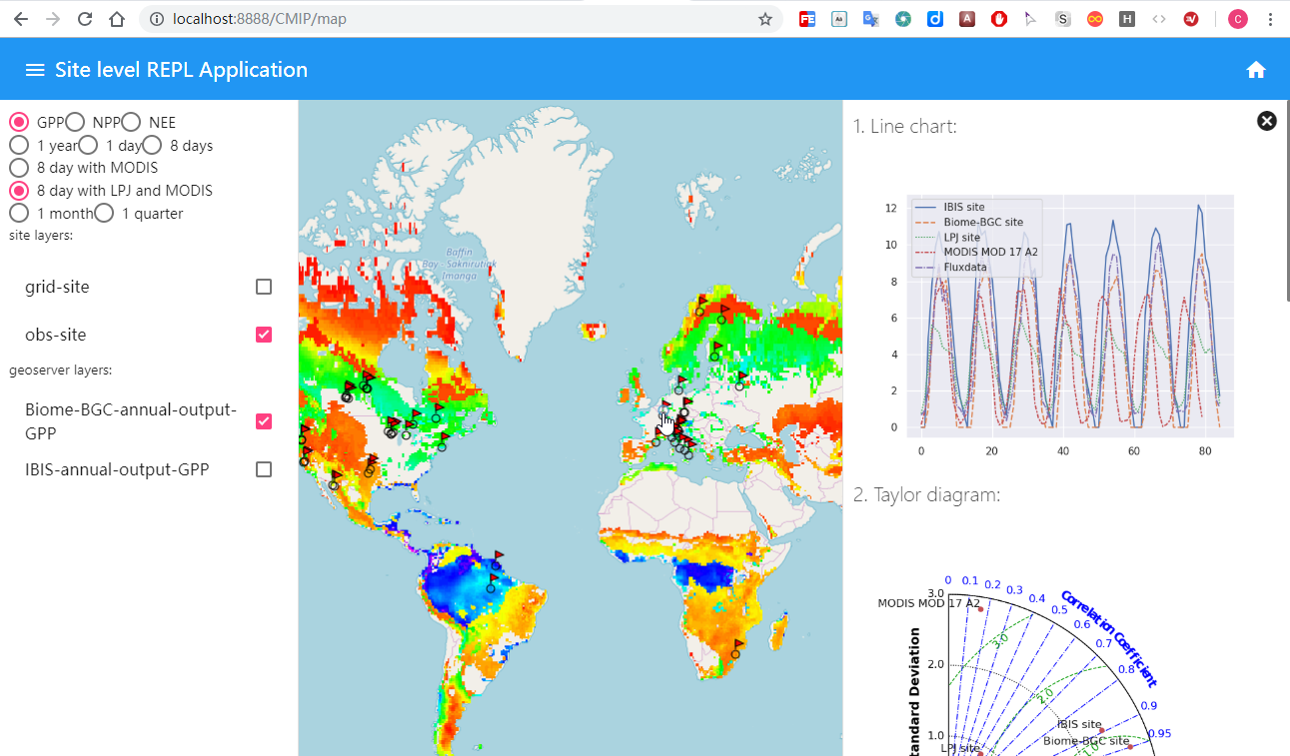
\includegraphics[width=.8\textwidth]{site-REPL}
    \caption{站点级对比结果查询应用}
    \label{fig:site-REPL}
\end{figure}

\section{实验案例}
GPP是评估。。,本文以同样的气象数据、和土壤数据驱动IBIS、Biome-BGC和LPJ,并参考MODIS GPP陆面产品,从单站点、多站点和全球三个维度分别对比四个模型的差异。
\subsection{基于单站点的时间趋势对比}


\subsection{基于植被功能类型的多站点差异性对比}
由于每个站点的观测数据时间范围不同,在不同站点上不能选取相同的时间范围,本研究取模拟时间范围(1982-2013年)和观测站点的最长公共时间区间,将每个站点的模拟结果与观测数据进行对比,最后按照植被功能类型进行统计,得到不同植被功能类型下不同模型模拟的GPP和观测的GPP的平均值差异及相关系数表,如图~\ref{fig:heatmap-GPP-coef}所示,在CSH、ENF、MF三种植被类型中,四个模型模拟的相关系数都在0.6以上,而对EBF的模拟效果最差,相关性在0.21以下,同时,如图~\ref{fig:heatmap-GPP-mean}所示,IBIS模拟的GPP整体偏高2倍左右,总体来看,Biome-BGC和LPJ的模拟结果比MODIS在各种植被功能类型上都更要准确,其中,Biome-BGC无论是从相关性还是从均值分布上模拟能力都是最好的。
按照表~\ref{tab:site-PFT-stat}所统计的8中站点植被功能类型,将129个站点的分类统计。

\begin{figure}[!htbp]
    \centering
    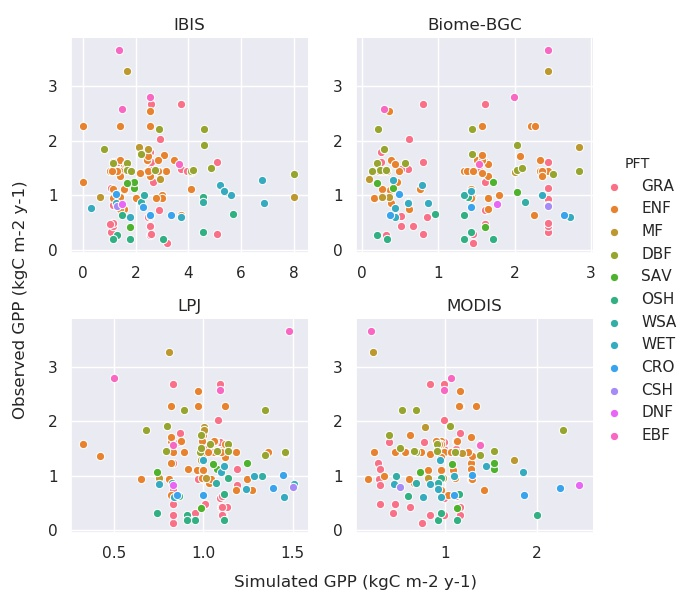
\includegraphics[width=1\textwidth]{scatter-GPP}
    \caption{129个站点GPP模拟值和观测值分布}
    \label{fig:api-gateway-children}
\end{figure}

% \begin{figure}[!htbp]
%     \centering
%     \subcaptionbox{相关系数\label{fig:heatmap-GPP-coef}}{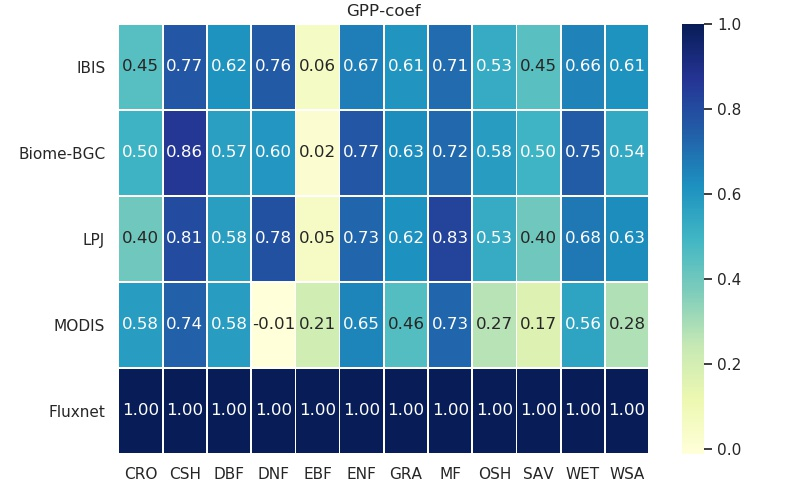
\includegraphics[width=.49\textwidth]{heatmap-GPP-coef}}
%     \hfill
%     \subcaptionbox{平均值\label{fig:heatmap-GPP-mean}}{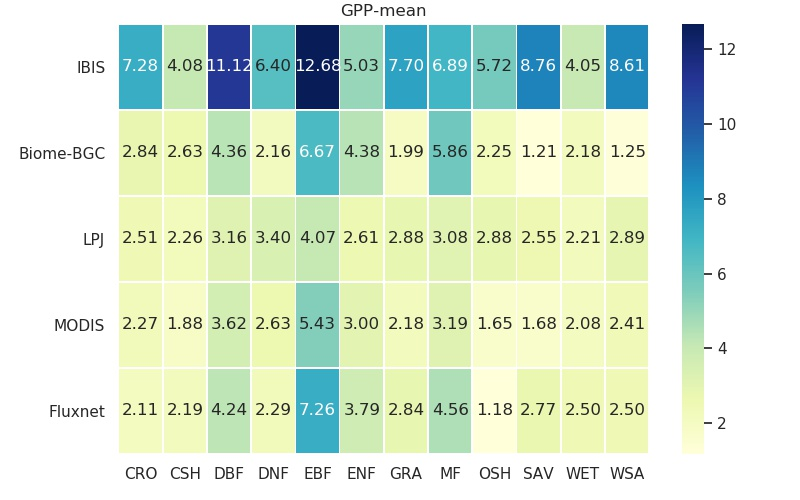
\includegraphics[width=.49\textwidth]{heatmap-GPP-mean}}
%     \caption{IBIS、Biome-BGC、LPJ和MODIS不同植被功能类型模拟的GPP相关系数和平均值对比}
%     \label{fig:heatmap-coef-mean}
% \end{figure}

\begin{table}
    \centering
    \caption{IBIS、Biome-BGC、LPJ、MODIS和Fluxnet的GPP统计指标}
    \label{tab:stats}
    \begin{threeparttable}
        \begin{tabular}{l|l|llllllllllll}
            \Xhline{1.5pt}
            模型 & 指标 & GRA & ENF & MF & DBF & SAV & OSH & WSA & WET & CRO & CSH & DNF & EBF \\
            \hline
            \multicolumn{2}{c}{站点数量} & 30 & 42 & 7 & 15 & 5 & 8 & 3 & 9 & 4 & 1 & 1 & 4 \\
            \Xhline{1.5pt}
            \parbox[t]{1mm}{\multirow{5}{*}{\rotatebox[origin=c]{-90}{\textbf{IBIS}}}} & mean & 7.70 & 5.03 & 6.89 & 11.12 & 8.76 & 5.72 & 8.61 & 4.05 & 7.28 & 4.08 & 6.40 & 12.68 \\
            & std & 4.05 & 3.08 & 3.16 & 4.67 & 4.66 & 3.89 & 4.11 & 2.55 & 4.36 & 2.88 & 2.98 & 1.96 \\
            & coef & 0.61 & 0.67 & 0.71 & 0.62 & 0.45 & 0.53 & 0.61 & 0.66 & 0.45 & 0.77 & 0.76 & 0.06 \\
            & rmsd & 6.70 & 2.87 & 3.18 & 8.62 & 7.56 & 5.92 & 6.94 & 3.25 & 6.49 & 2.19 & 4.54 & 6.89 \\
            & nse & -27.24 & -1.29 & -0.36 & -14.30 & -176.24 & -91.04 & -10.81 & -2.99 & -10.69 & 0.03 & -7.49 & -47.69 \\
            \hline
            \parbox[t]{1mm}{\multirow{5}{*}{\rotatebox[origin=c]{-90}{\textbf{Biome-BGC}}}} & mean & 1.99 & 4.38 & 5.86 & 4.36 & 1.21 & 2.25 & 1.25 & 2.18 & 2.84 & 2.63 & 2.16 & 6.67 \\
            & std & 1.35 & 2.93 & 2.72 & 1.72 & 0.68 & 1.82 & 0.68 & 1.42 & 2.31 & 3.06 & 1.50 & 1.08 \\
            & coef & 0.63 & 0.77 & 0.72 & 0.57 & 0.50 & 0.58 & 0.54 & 0.75 & 0.50 & 0.86 & 0.60 & 0.02 \\
            & rmsd & 2.53 & 2.91 & 2.93 & 3.19 & 2.78 & 2.31 & 2.17 & 2.12 & 3.33 & 2.09 & 1.39 & 2.42 \\
            & nse & -0.10 & -1.15 & -0.32 & 0.09 & -1.68 & -6.96 & -0.18 & -0.08 & -1.68 & -0.18 & 0.23 & -1.63 \\
            \hline
            \parbox[t]{1mm}{\multirow{5}{*}{\rotatebox[origin=c]{-90}{\textbf{LPJ}}}} & mean & 2.88 & 2.61 & 3.08 & 3.16 & 2.55 & 2.88 & 2.89 & 2.21 & 2.51 & 2.26 & 3.40 & 4.07 \\
            & std & 2.14 & 2.40 & 2.40 & 1.96 & 1.44 & 1.85 & 1.62 & 2.03 & 2.06 & 2.45 & 2.55 & 0.40 \\
            & coef & 0.62 & 0.73 & 0.83 & 0.58 & 0.40 & 0.53 & 0.63 & 0.68 & 0.40 & 0.81 & 0.78 & 0.05 \\
            & rmsd & 2.98 & 2.39 & 2.68 & 3.11 & 2.50 & 2.47 & 1.61 & 1.95 & 2.13 & 1.45 & 2.14 & 3.80 \\
            & nse & -3.40 & -0.01 & 0.08 & 0.10 & -6.22 & -11.35 & 0.37 & 0.12 & -0.25 & 0.53 & -0.79 & -7.15 \\
            \hline
            \parbox[t]{1mm}{\multirow{5}{*}{\rotatebox[origin=c]{-90}{\textbf{MOD17A2}}}} & mean & 2.18 & 3.00 & 3.19 & 3.62 & 1.68 & 1.65 & 2.41 & 2.08 & 2.27 & 1.88 & 2.63 & 5.43 \\
            & std & 1.77 & 2.66 & 2.56 & 2.27 & 0.93 & 1.42 & 1.29 & 1.69 & 1.90 & 2.22 & 1.73 & 1.54 \\
            & coef & 0.46 & 0.65 & 0.73 & 0.58 & 0.17 & 0.27 & 0.28 & 0.56 & 0.58 & 0.74 & -0.01 & 0.21 \\
            & rmsd & 2.58 & 2.44 & 2.98 & 2.82 & 2.59 & 1.59 & 2.09 & 2.09 & 1.88 & 1.61 & 2.36 & 2.71 \\
            & nse & -0.47 & -0.09 & -0.34 & 0.11 & -0.75 & -1.85 & -0.08 & -0.08 & 0.09 & 0.47 & -1.25 & -3.27 \\
            \hline
            \parbox[t]{1mm}{\multirow{2}{*}{\rotatebox[origin=c]{-90}{\textbf{FLUXNET}}}} & mean & 2.84 & 3.79 & 4.56 & 4.24 & 2.77 & 1.18 & 2.50 & 2.50 & 2.11 & 2.19 & 2.29 & 7.26 \\
            & std & 2.50 & 2.54 & 3.29 & 3.40 & 2.24 & 1.04 & 2.02 & 2.12 & 2.12 & 2.26 & 1.59 & 1.55 \\
            \Xhline{1.5pt}
        \end{tabular}
        \begin{tablenotes}
            \footnotesize
            \item 观测数据来源于FLUXNET,共129个站点。
        \end{tablenotes}
    \end{threeparttable}
\end{table}

% \begin{figure}[!htbp]
%     \centering
%     \subcaptionbox{OSH\label{fig:taylor-GPP-OSH}}{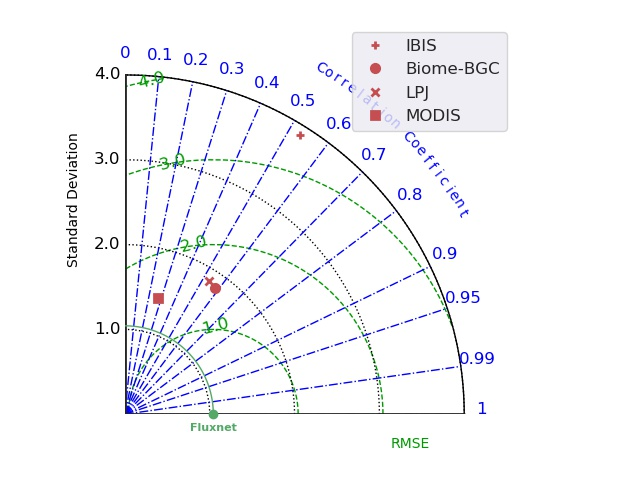
\includegraphics[width=.48\textwidth]{taylor-GPP-OSH}}
%     \hfill
%     \subcaptionbox{CSH\label{fig:taylor-GPP-CSH}}{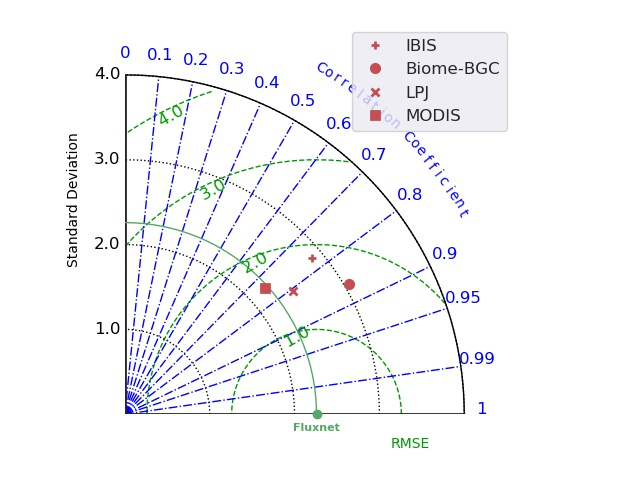
\includegraphics[width=.48\textwidth]{taylor-GPP-CSH}} \\
%     \subcaptionbox{DBF\label{fig:taylor-GPP-DBF}}{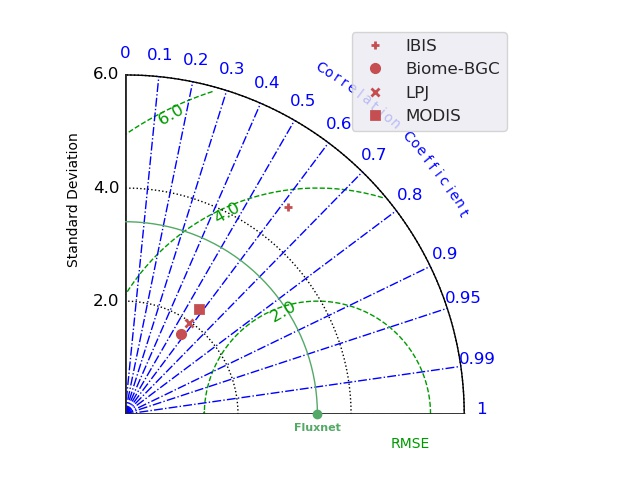
\includegraphics[width=.48\textwidth]{taylor-GPP-DBF}}
%     \hfill
%     \subcaptionbox{EBF\label{fig:taylor-GPP-EBF}}{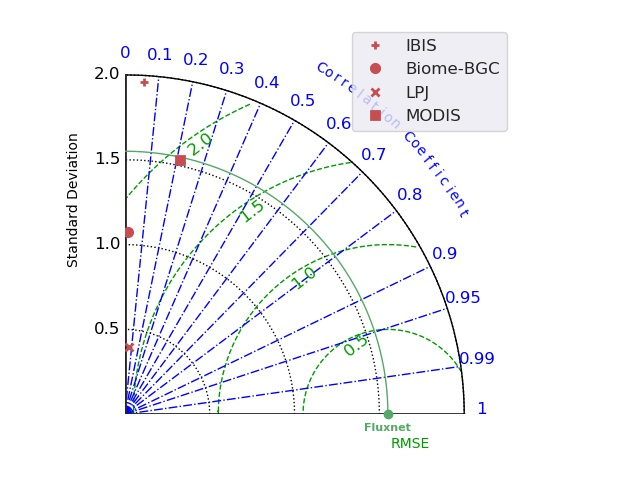
\includegraphics[width=.48\textwidth]{taylor-GPP-EBF}} \\
%     \subcaptionbox{DNF\label{fig:taylor-GPP-DNF}}{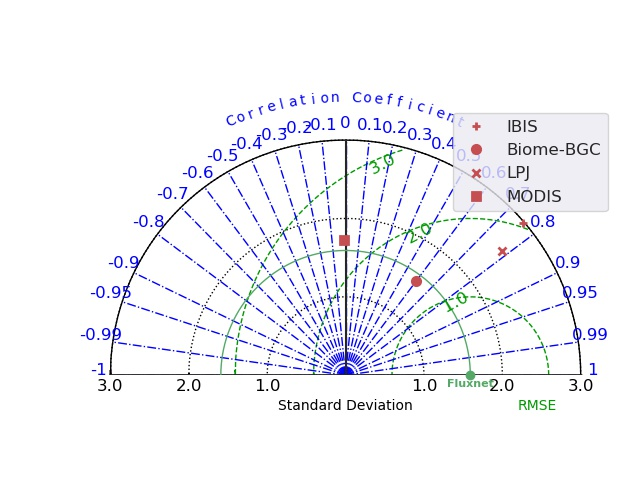
\includegraphics[width=.48\textwidth]{taylor-GPP-DNF}} 
%     \hfill
%     \subcaptionbox{ENF\label{fig:taylor-GPP-ENF}}{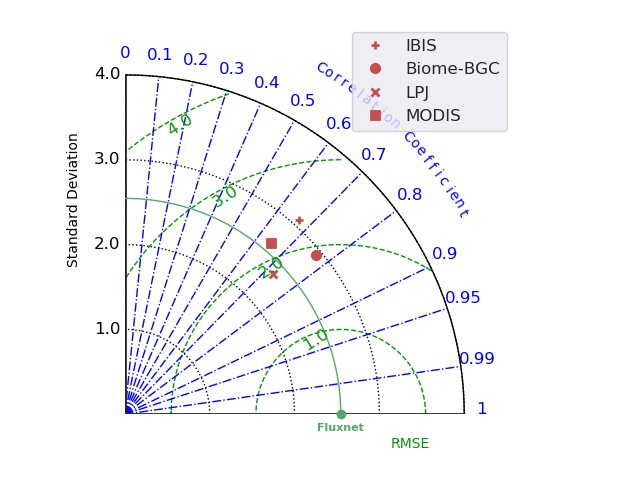
\includegraphics[width=.48\textwidth]{taylor-GPP-ENF}} \\
%     \subcaptionbox{GRA\label{fig:taylor-GPP-GRA}}{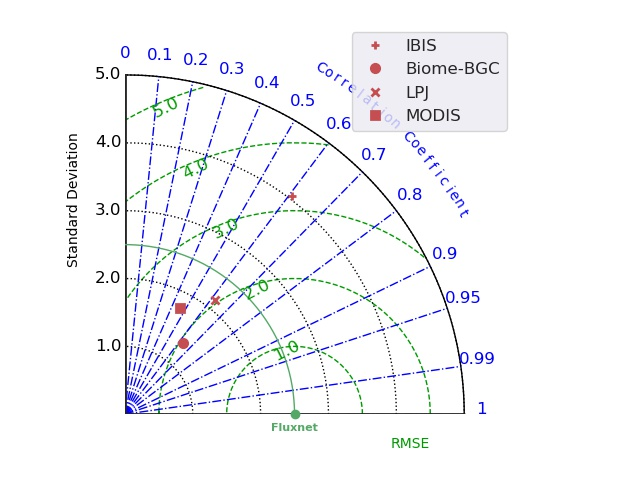
\includegraphics[width=.48\textwidth]{taylor-GPP-GRA}}
%     \hfill
%     \subcaptionbox{SAV\label{fig:taylor-GPP-SAV}}{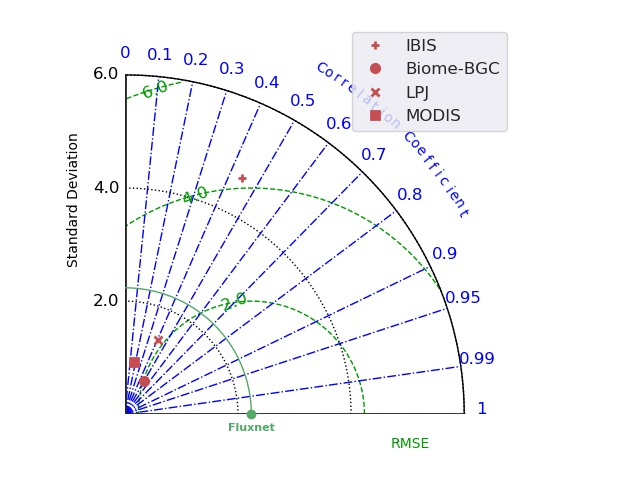
\includegraphics[width=.48\textwidth]{taylor-GPP-SAV}}
%     % \hfill
%     % \subcaptionbox{WSA\label{fig:taylor-GPP-WSA}}{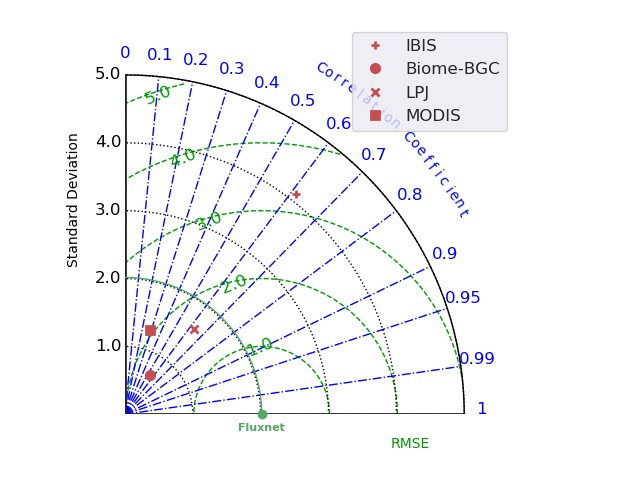
\includegraphics[width=.48\textwidth]{taylor-GPP-WSA}} 
%     % \hfill
%     % \subcaptionbox{CRO\label{fig:taylor-GPP-CRO}}{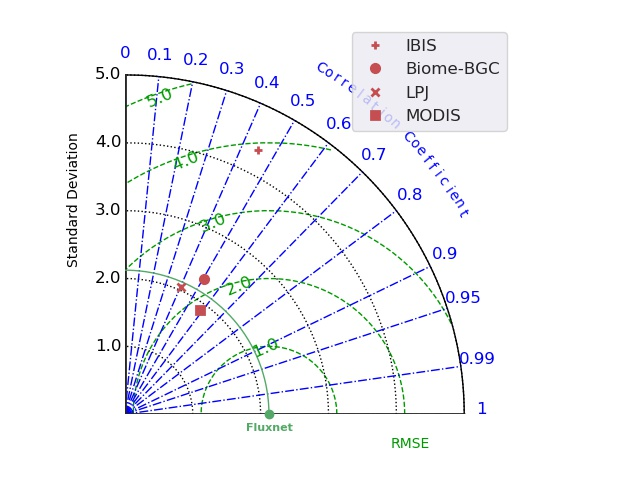
\includegraphics[width=.48\textwidth]{taylor-GPP-CRO}}
%     % \subcaptionbox{MF\label{fig:taylor-GPP-MF}}{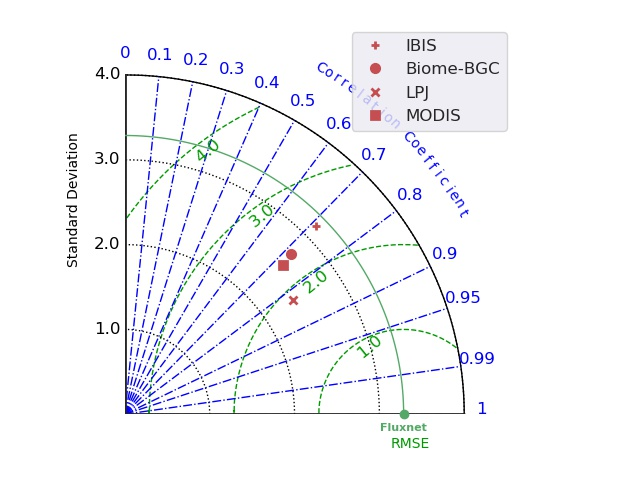
\includegraphics[width=.48\textwidth]{taylor-GPP-MF}} \\
%     % \subcaptionbox{WET\label{fig:taylor-GPP-WET}}{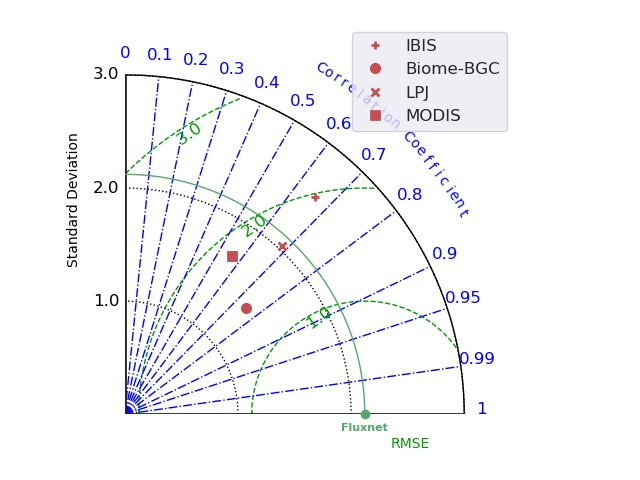
\includegraphics[width=.48\textwidth]{taylor-GPP-WET}}
%     \caption{IBIS、Biome-BGC、LPJ和MODIS计算的GPP不同植被功能类型的雷达图}
%     \label{fig:GPP-cmp-taylor}
% \end{figure}


\subsection{基于全球网格点的时空格局对比}
\subsubsection{时间变化对比}
本文基于全球范围内划分的网格点的模拟结果,以MOD17A2的模拟结果进行交叉对比,如图~\ref{fig:GPP-annual}三个模型模拟的GPP都承缓慢上升趋势,其中Biome-BGC的结果和MODIS的模拟结果最为接近,而IBIS整体偏高,LPJ整体偏低。4个模型模拟的GPP季节分布规律如图~\ref{fig:GPP-monthly},不论南北半球都是夏季GPP升高,冬季GPP降低。

\begin{figure}[!htbp]
    \centering
    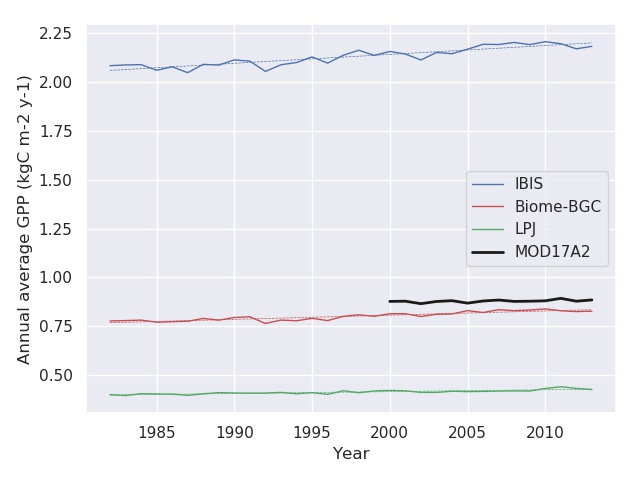
\includegraphics[width=.8\textwidth]{GPP-annual}
    \caption{IBIS、Biome-BGC、LPJ和MODIS模拟的GPP的年际变化趋势}
    \label{fig:GPP-annual}
\end{figure}

\begin{figure}[!htbp]
    \centering
    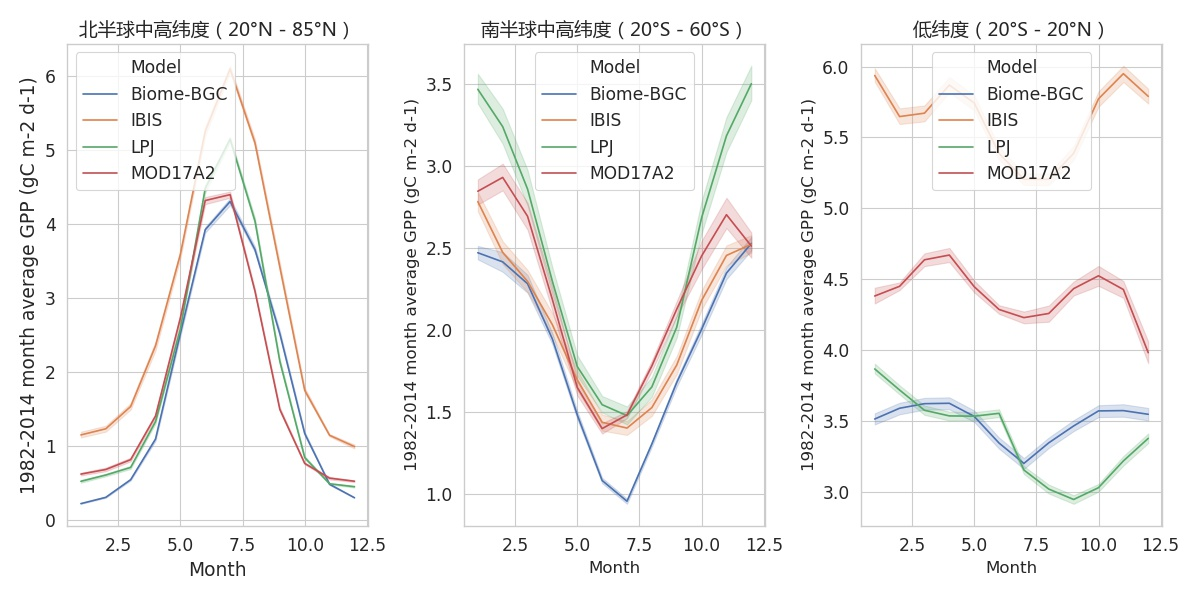
\includegraphics[width=1\textwidth]{GPP-monthly}
    \caption{IBIS、Biome-BGC、LPJ和MODIS模拟的GPP的季节变化规律}
    \label{fig:GPP-monthly}
\end{figure}


\subsubsection{空间格局对比}
% TODO 全球总GPP
从空间格局上来看,Biome-BGC模拟结果与MOD17A2的结果最为接近,而IBIS全球范围内都偏高,而LPJ模拟的整体稍微偏低。从纬度的分布上来看,如图~\ref{fig:GPP-lat},GPP的分布存在着明显的维度规律,在低纬度GPP最高,在低纬度GPP偏低。

\begin{figure}[!htbp]
    \centering
    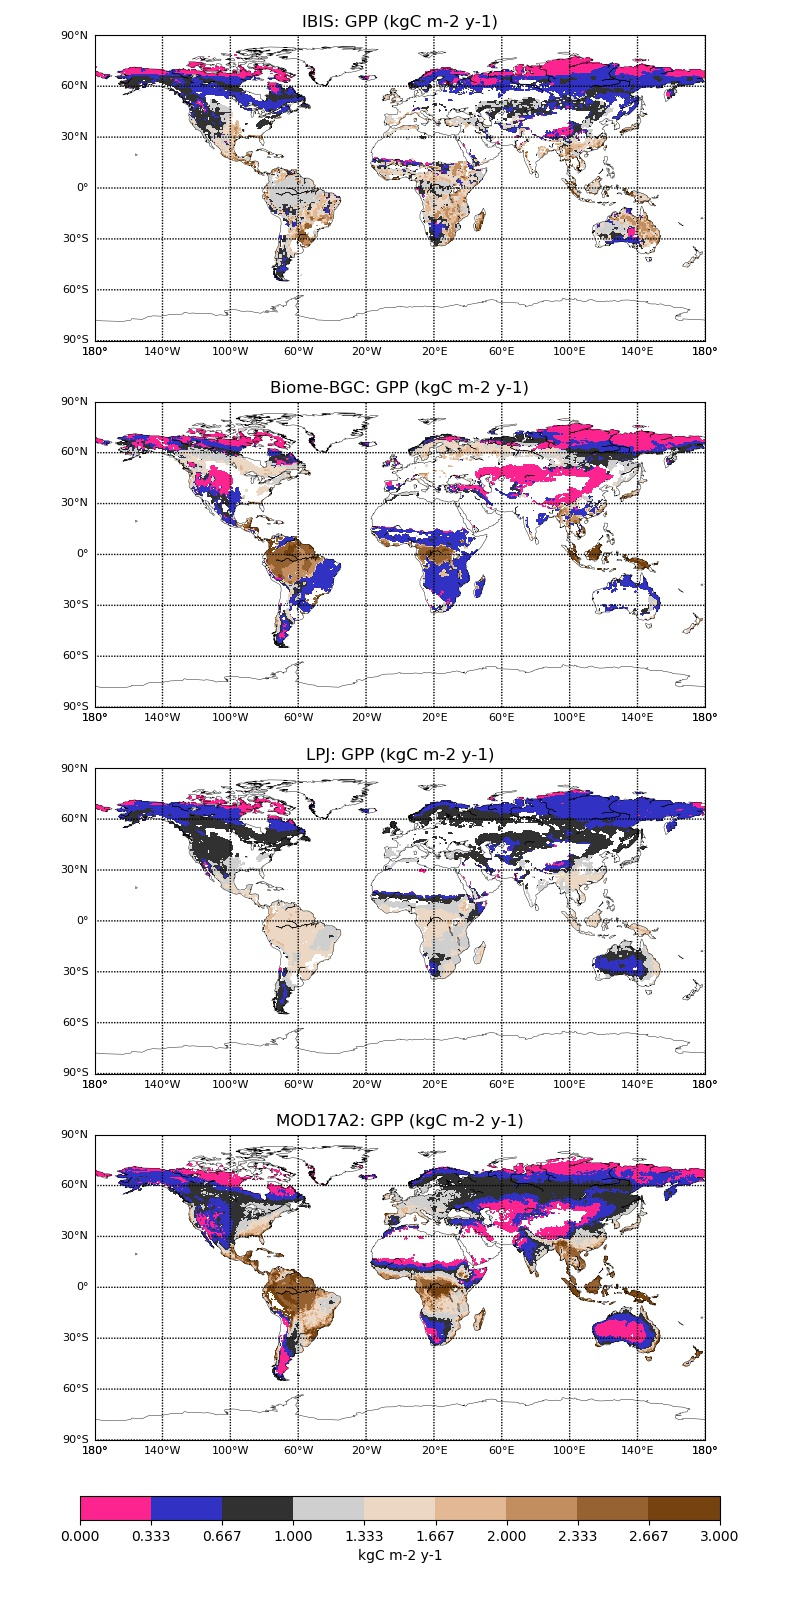
\includegraphics[width=.8\textwidth]{GPP}
    \caption{IBIS、Biome-BGC、LPJ和MODIS的GPP的空间分布格局对比}
    \label{fig:GPP}
\end{figure}

\begin{figure}[!htbp]
    \centering
    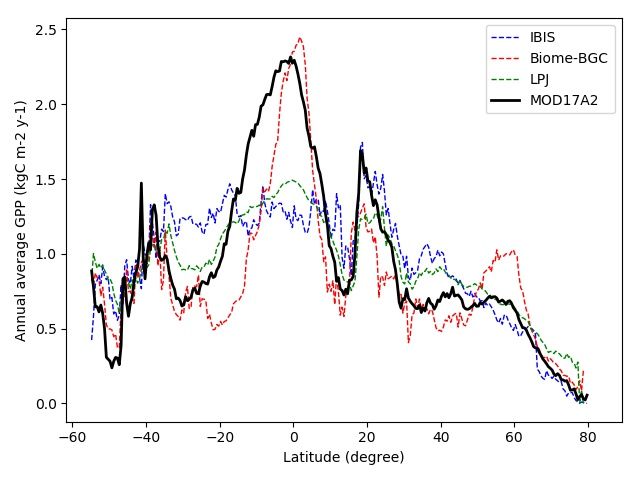
\includegraphics[width=1\textwidth]{GPP-lat}
    \caption{IBIS、Biome-BGC、LPJ和MODIS的GPP的纬向变化规律}
    \label{fig:GPP-lat}
\end{figure}